A área de pesquisa conhecida como \textit{aprendizado de máquina} permeia o cotidiano humano provendo auxílio em diversas áreas, como bioinformática, visão computacional e recomendação de conteúdo - entre outras \cite{journals/bmcbi/WangLLXHXL14,conf/nips/KrizhevskySH12,reference/rsh/RicciRS11}.
Uma das principais tarefas de algoritmos de aprendizado de máquina é a de classificação de dados.
Ela busca associar objetos de interesse, \textit{exemplos}\footnote{
Os termos adotados para a representação inequívoca de conceitos importantes estão marcados em itálico em sua definição/primeira ocorrência.
Em tempo, optou-se pela grafia das palavras em português quando existente (\textit{ranqueamento}, por exemplo, introduzida na Seção \ref{contribuicao}) e pelas contrações facultativas mais comuns de preposição e artigo indefinido, prescritas na norma padrão da língua portuguesa \cite{lima1973gramatica,academia2004vocabulario}.
}, a classes.
Esse tipo de categorização é típica do grupo de tarefas denominado \textit{aprendizado supervisionado}, pois requer, usualmente, a supervisão de um especialista - chamado \textit{oráculo} no contexto deste trabalho.
Após um esforço suficiente de supervisão na categorização de um \textit{conjunto} de exemplos para treinamento, torna-se possível a predição da classe de novos exemplos.
Esse é o objetivo final da tarefa de classificação.
% agora retoma tudo o que foi dito e resume em três requisitos
Nesse contexto, o desempenho preditivo de algoritmos de aprendizado depende do cumprimento de pelo menos três 
requisitos:
\begin{itemize}
 \item a \textbf{amostragem} de dados para a construção do conjunto de treinamento deve ser representativa do problema em questão;
 \item o processo de \textbf{categorização} desses dados deve disponibilizar conhecimento suficiente para o aprendizado da tarefa desejada; e,
 \item o algoritmo de \textbf{aprendizado} deve ser adequado ao domínio do problema.
% tempo, viés, escalabilidade etc.
\end{itemize}
Esses requisitos podem ser cumpridos de acordo com o ambiente de aprendizado de máquina ilustrado na Figura \ref{aprsup}.
\begin{figure}
  \setlength{\unitlength}{1.0cm}
  \centering
    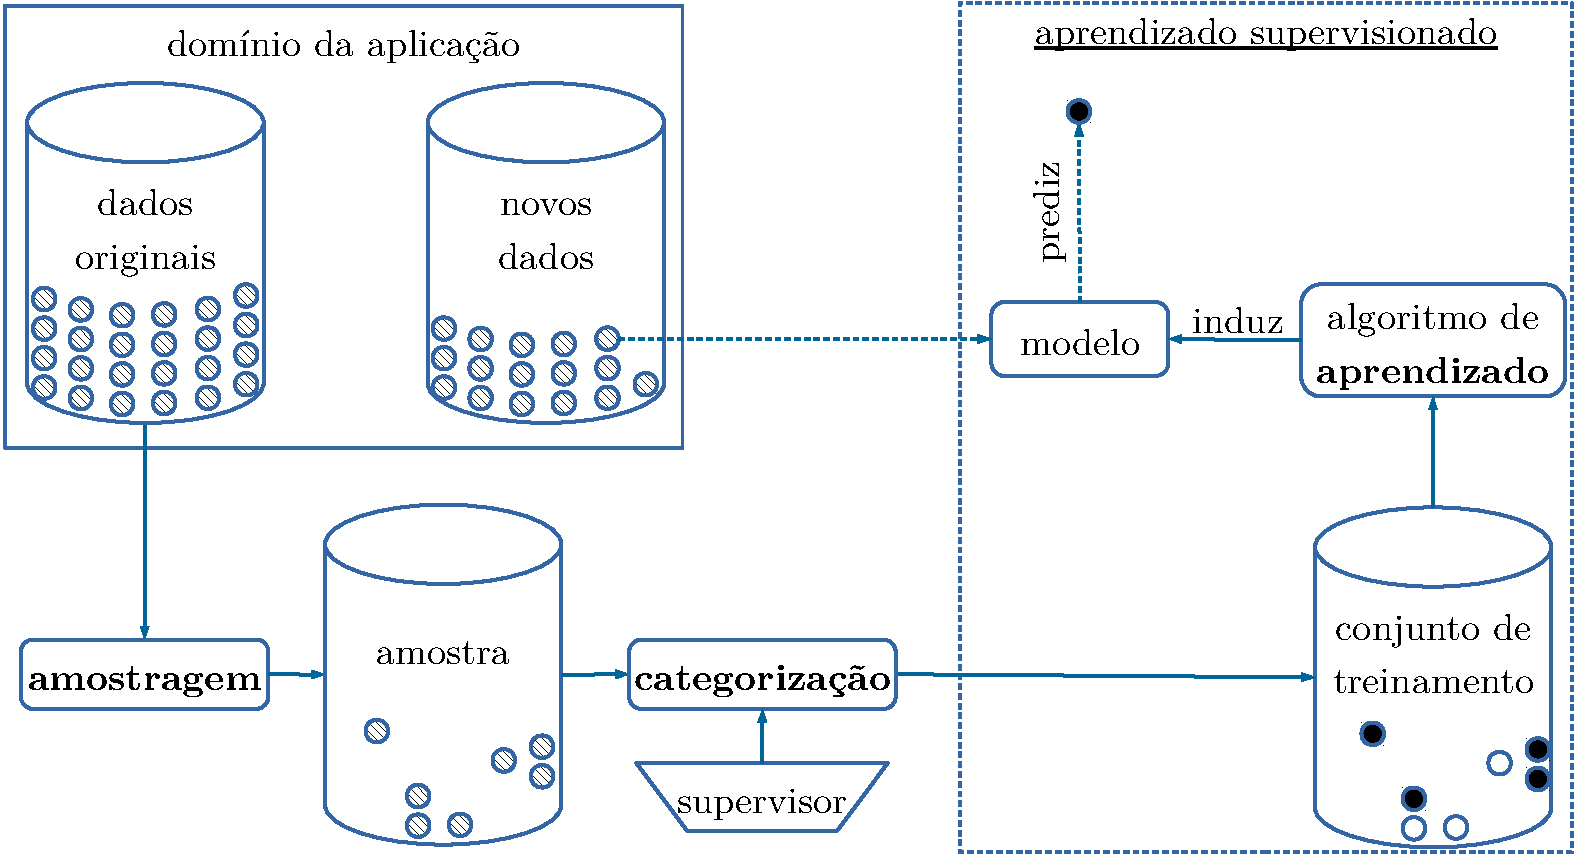
\includegraphics[scale=0.5]{apsup.pdf}
  \caption[Esquema de aprendizado supervisionado.]{Esquema de aprendizado supervisionado e componentes externos.}
  \label{aprsup}
\end{figure}
Uma amostra dos exemplos (ou todos) disponíveis no domínio do problema é classificada de acordo com as classes atribuídas por um supervisor.
O resultado é o conjunto de dados de treinamento para a geração de um \textit{modelo} de classificação.

\section{Motivação}\label{motiv}
Assumindo-se a disponibilidade de infraestrutura computacional, a necessidade de esforço humano pode se tornar o maior obstáculo para um projeto de aprendizado supervisionado ser bem sucedido.
Esse esforço pode ser necessário em pelo menos duas perspectivas de atuação que abrangem os passos em destaque na Figura \ref{aprsup}:
% sobre enumerações: http://www.portaleducacao.com.br/educacao/artigos/46190/pontos-fundamentais-da-gramatica-enumeracoes
\begin{itemize}
\item no projeto do sistema, tanto na escolha da forma de {amostragem} quanto na determinação do algoritmo de {aprendizado} mais adequado ao problema; e,
\item durante a {categorização} dos dados, normalmente realizada por um ou mais supervisores humanos.
\end{itemize}
No primeiro caso, um especialista em aprendizado de máquina toma decisões relacionadas à implementação do sistema.
No segundo caso, especialistas no domínio do problema fazem a \textit{rotulação}, ou seja, atribuem rótulos informando a classe de cada objeto de interesse.
As atividades realizadas nos dois momentos podem ter um custo elevado.

O custo de rotulação pode ser facilmente contabilizado pela quantidade de rótulos necessários para a construção do conjunto de treinamento.
Por outro lado, o custo das decisões do especialista é de estimação mais incerta, pois envolve o esforço despendido no processo de escolha e suas possíveis consequências.
Quanto menor a confiança desse especialista na escolha do processo de amostragem ou do algoritmo de aprendizado, maiores as chances da aplicação incorrer em custos adicionais ou prejuízo no desempenho preditivo futuro.
% 'tratar-se de' é sempre singular quando não é doença
Portanto, custo de rotulação e custo decorrente de inadequação do sistema à tarefa desejada são dois aspectos importantes - quando se deseja garantir a viabilidade financeira de uma aplicação.

Além da questão econômica, o desempenho do sistema também depende das decisões tomadas na fase de projeto.
Acurácia preditiva e tempo de processamento, por exemplo, são diretamente afetados pela escolha do algoritmo de aprendizado.
Ademais, a qualidade dos dados amostrados e o próprio viés da \textit{estratégia} de amostragem escolhida também influenciam diretamente no desempenho.
Logo, a definição do par \textit{estratégia-algoritmo} ideal para um dado problema tem um papel central no projeto de um sistema de aprendizado supervisionado como aquele exposto previamente na Figura \ref{aprsup}.
A necessidade de definição desse par motiva a realização de uma pesquisa que se aprofunde além da simples comparação de poucas estratégias de amostragem, com mais do que somente um algoritmo de aprendizado e mais do que uma dúzia de conjuntos de dados - como tem sido feito na literatura \cite{journals/corr/EvansAA14a,conf/emnlp/SettlesC08,journals/ml/ScheinU07,conf/ecml/KornerW06}.
% They have a restricted scope, such as focus on strategies for a particular 
% classification algorithm \cite{journals/ml/ScheinU07}, 
% specific tasks \cite{conf/emnlp/SettlesC08} or 
% a single family of strategies \cite{conf/ecml/KornerW06}.
% % http://arxiv.org/pdf/1408.1319.pdf
% In a recent comparison, active learning failed in \textit{more often than not}, according to
% \cite{journals/corr/EvansAA14a}.
% The authors used two strategies (Uncertainty Sampling and QBC) and
% four algorithms (Logistic Regression, Quadratic Discriminant Analysis,
% Random Forest and Support Vector Machines).
% Therefore, we believe more comprehensive studies and experiments attesting the active learning feasibility are necessary.

O cenário de \textit{aprendizado ativo} é explorado neste trabalho visando abordar o problema da redução do custo de rotulação (Seção \ref{aprendizado-ativo}).
Apenas os exemplos mais relevantes do conjunto de dados são escolhidos.
No cenário específico desta tese, que será detalhado na Seção \ref{desccen}, o conjunto de dados não rotulados é chamado \ing{reserva de exemplos}{pool}.
Nesse contexto, o conjunto de treinamento cresce enquanto houver \textit{orçamento} - seguindo o ciclo \mbox{\textit{consulta} \MVRightarrow\phantom{i}\textit{rotula} \MVRightarrow\phantom{i}\textit{induz}} 
apresentado na Figura \ref{apsupal}.
\begin{figure}
  \setlength{\unitlength}{1.0cm}
  \centering
    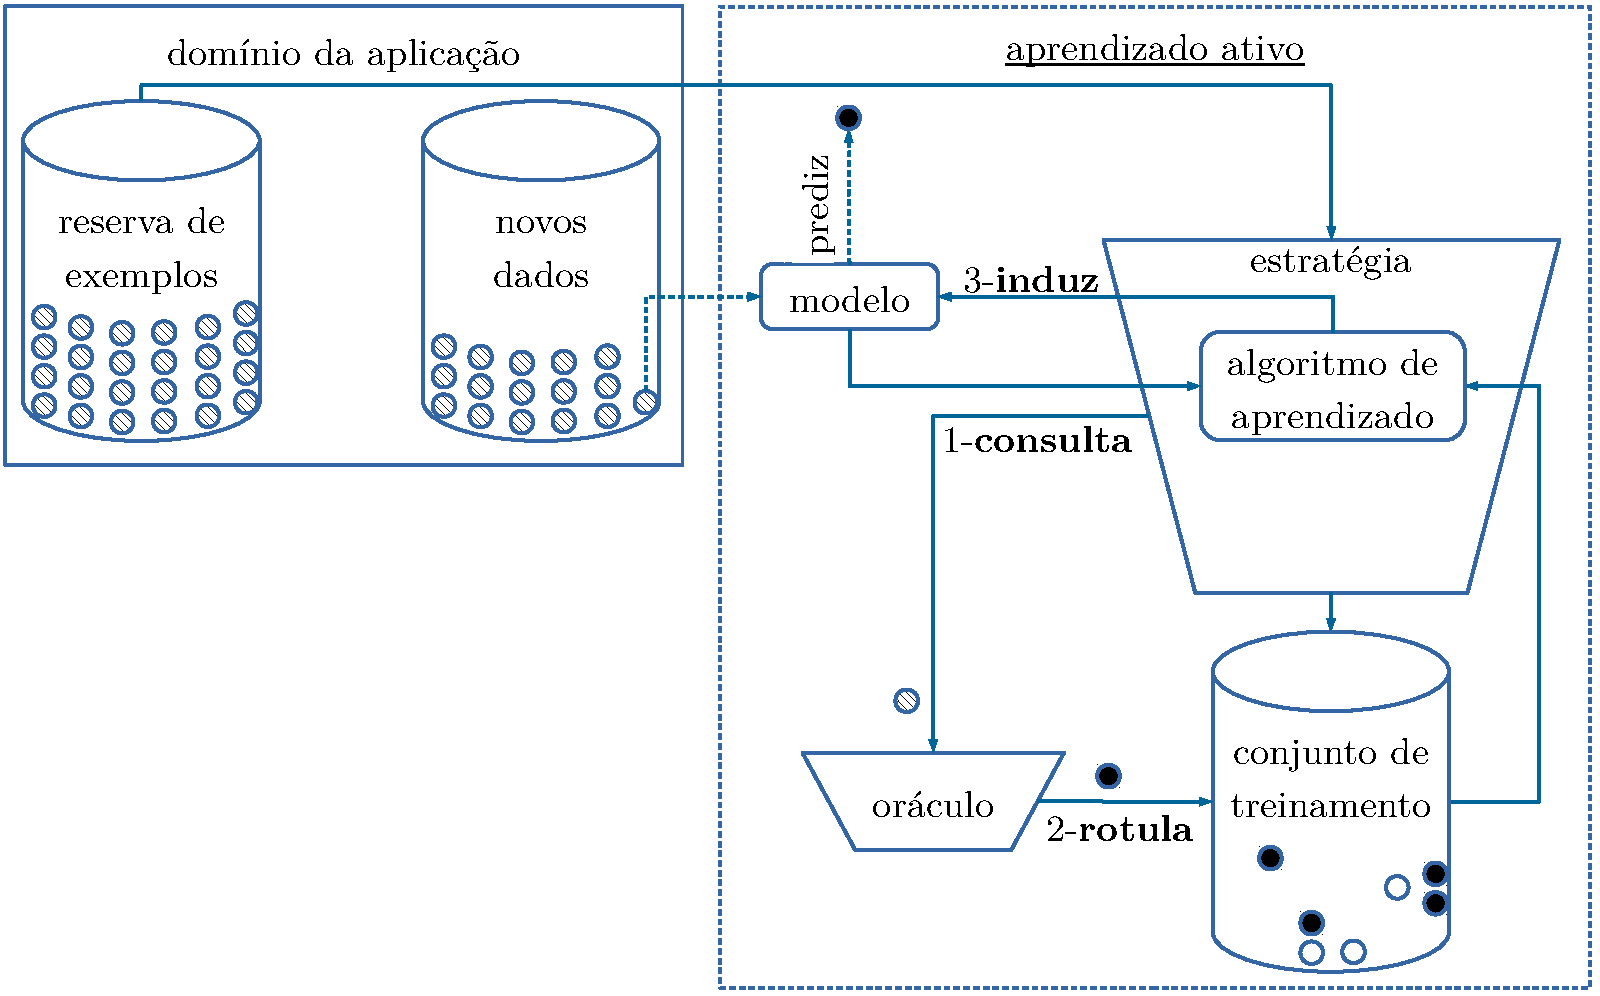
\includegraphics[scale=0.5]{apsupal.pdf}
  \caption{Esquema de aprendizado ativo.}
  \label{apsupal}
\end{figure}
Consequentemente, a administração do custo de rotulação passa a ser atribuição de uma estratégia de amostragem ativa.
Para fins experimentais, o orçamento indica o número de \textit{consultas} permitidas.

Finalmente, a questão da possível inadequação do algoritmo de aprendizado ao domínio do problema permanece em aberto.
Assim, a indução de um modelo adequado depende da escolha do par estratégia-algoritmo, ou apenas da estratégia, no caso excepcional em que tenha sido adotada uma estratégia sem \textit{aprendiz} (Capítulo \ref{contexto}).
Uma estratégia sem aprendiz é uma estratégia que não necessita de um algoritmo de aprendizado para realizar as consultas.
% , ou seja, que não recorra aos modelos gerados por algoritmos de aprendizado.
A motivação para a pesquisa em ambas componentes do par estratégia-algoritmo é dada nas seções \ref{ee} e \ref{ea}.

\subsection{Escolha da estratégia}\label{ee}
A existência de diversas estratégias na literatura de aprendizado ativo coloca o especialista em aprendizado de máquina diante de uma escolha para a qual não há um critério claro.
A principal dificuldade advém da impossibilidade de comparação dos desempenhos dessas diferentes abordagens 
% para um determinado conjunto de dados 
sem incorrer em custos de rotulação.
Isso se deve ao fato de que a qualidade das consultas é dada, em última instância, pela acurácia do modelo induzido.
Sendo a indução somente possível com a presença dos rótulos e esses são provenientes da interação estratégia-oráculo, tem-se um paradoxo:
a escolha da estratégia depende dos rótulos que, por sua vez, dependem da estratégia.

Na literatura da área, a escolha da estratégia a ser utilizada tem sido quase arbitrária, tendendo a se concentrar no uso da mais simples - a \textit{amostragem por incerteza}.
Essa preferência foi reportada numa competição de aprendizado ativo \cite{journals/jmlr/GuyonCDL11} - conforme ilustrado na Figura \ref{compet}.
% Nessa competição também prevaleceu a omissão de estratégias possivelmente mais efetivas (Capítulo \ref{experimentos}).
\begin{figure}
	\centering
	\includestandalone[mode=buildmissing]{images/barras}
	\caption[Frequência de uso de estratégias na competição de aprendizado ativo.]{Frequência de uso de estratégias na competição de aprendizado ativo - descritas na Seção \ref{secestrategias}.
	Alguns participantes adotaram mais de uma estratégia.
	\textit{Adaptado de \citeonline{journals/jmlr/GuyonCDL11}.}}
	\label{compet}
\end{figure}
% challenge:
% global_score = (ALC-Arand)/(Amax-Arand)       Amax = 1
% semi-supervised learning is needed to achieve good performance in the first part of the learning curve
% (usar ou não semisupervised é um problema à parte, que faz parter do learner, não da estratégia; classificadores semisupervisionados são melhores, mas não é isso que se está avaliando quando se comparam estratégias; ensembles, feature selection e SMOTE também ajudam e nem por isso precisam ser empregados na comparação de estratégias)
Em consonância com esse panorama está a ausência de estudos comparativos abrangentes que possam guiar o especialista na definição da estratégia de consulta a ser empregada - até onde o conhecimento do autor desta tese permite dizer.
Consequentemente, a maneira ideal de redução do custo de rotulação ainda é um problema em aberto.

\subsection{Escolha do algoritmo}\label{ea}
A questão da escolha do algoritmo de aprendizado para a indução de modelos de classificação é análoga à questão da escolha da estratégia.
A escolha do algoritmo é definida neste texto da seguinte forma: seleção \textit{manual} - baseada em experiência pessoal de experimentos anteriores do especialista; ou, seleção \textit{automática} - baseada em sistemas de recomendação, como o \textit{meta-aprendizado} (Apêndice \ref{apmeta}).
% 'meta-aprendizado' é pouco mencionado aqui. Ele só vai ser abreviado depois que for definido no capítulo correspondente, para evitar confusão aqui com outras siglas.

Usualmente, ambas abordagens (manual e automática) empregam validação cruzada durante a comparação de algoritmos candidatos \cite{conf/pakdd/BouckaertF04,books/daglib/0022052}.
Isso as torna mais aplicáveis ao cenário em que o conjunto de treinamento já esteja construído.
Entretanto, no cenário de aprendizado ativo, a rotulação é um processo em andamento, assim como seu conjunto de treinamento resultante.
Tal característica impede que o especialista disponha da importante fonte de informação que um conjunto de treinamento completo poderia representar.
Reduz-se, assim, a quantidade de informações disponíveis para decisões bem fundamentadas.
Logo, além da escolha da estratégia ser incerta pela falta de critérios, conforme visto na Seção \ref{ee}, a escolha do algoritmo mais adequado para o papel de aprendiz também carece de melhores fundamentos.

\section{Hipóteses}\label{hipoteses}
O teorema conhecido como \sigla{NFL}{\textit{No Free Lunch}} permite afirmar que nenhum algoritmo de aprendizado pode ser o mais adequado para todos os domínios \cite{conf/icml/Schaffer94}.
A mesma afirmação é válida para algoritmos de otimização \cite{journals/tec/DolpertM97} e, consequentemente, válida para estratégias de amostragem ativa.
Assim, é garantida a existência da questão da escolha no presente cenário do ponto de vista teórico.
A razão de uma estratégia poder ser entendida como um procedimento de otimização é ela consistir na busca pela melhor sequência de exemplos dentro das possibilidades que a reserva de exemplos e o orçamento permitem.
Dessa forma, é possível definir o contexto para as hipóteses desta tese:
\textit{cada estratégia tem um viés de amostragem, normalmente dependente de um viés de aprendizado, que favorece determinados domínios de problemas e prejudica outros}.
% - analogamente ao viés de aprendizado de um algoritmo de classificação passiva. 
Diante desse cenário, e considerando a motivação apresentada previamente
na Seção \ref{motiv}, duas hipóteses foram formuladas.
A Hipótese I corresponde à principal tese defendida neste trabalho:
% enumeração seguida de ponto final pede inicial maiúscula

\noindent\fbox{\parbox{.98\textwidth}{
É possível explorar relações entre conjuntos de dados e 
\textit{algoritmos de aprendizado, estratégias de aprendizado ativo ou pares de ambos}, de maneira que seja possível escolher abordagens para essas duas componentes que resultem num melhor desempenho preditivo que uma escolha arbitrária.}}\\

A Hipótese II, secundária, supõe que \textit{a presença ou tipo do viés de aprendizado podem ser controlados durante o processo de rotulação, aumentando o desempenho preditivo}.
% a concordância entre o verbo e o sujeito depende do valor da conjunção 'ou' (inclusivo ou exclusivo) 

A Seção \ref{intropropostas} contém a proposta de investigação das hipóteses.

\section{Proposta}\label{intropropostas}
A proposta desta tese é a investigação de alternativas para facilitar a escolha da estratégia de amostragem e/ou seu correspondente algoritmo de aprendizado mais adequados para um conjunto de dados.
Uma particularidade do cenário de aprendizado ativo é que o subconjunto inicial de exemplos rotulados é vazio ou pequeno demais para escolhas apropriadas.
% 'alternativas' inclui análise de nichos, HTU e culmina em MTL;
Assim, o resultado esperado da investigação é que a escolha da estratégia, do algoritmo ou do par estratégia-algoritmo possa ser realizada de uma maneira mais objetiva que a convencional, induzindo modelos com melhor acurácia preditiva para um dado orçamento.
% Isso será atestado vencendo a escolha arbitrária (majoritário).

% \subsection{Investigação}\label{invest}
A investigação concentra-se nos seguintes objetivos, em ordem decrescente do grau de participação requerida do especialista que hipoteticamente usufruiria dos resultados:
\begin{itemize}
   \item identificação de nichos de problemas onde a utilização de certas estratégias seja adequada - teste qualitativo da Hipótese I;
   \item desenvolvimento de uma estratégia capaz de suprimir a influência do algoritmo de aprendizado na fase de rotulação, quando seu uso for prejudicial - teste da Hipótese II; e,
   \item teste inicial de uma estratégia que poderia ser chamada \textit{aprendizado meta-ativo}\footnote{Note-se a distinção entre \textit{aprendizado meta-ativo} e \textit{meta-aprendizado ativo} \cite{conf/ijcnn/SousaPSL13} explanada na Seção \ref{sec:ama}.} (meta-aprendizado aplicado a aprendizado ativo) capaz de escolher (e trocar) o algoritmo antes de (e durante) o aprendizado - teste quantitativo das Hipóteses I e II. 
\end{itemize}
Os meios escolhidos para atingir essas metas são: revisão bibliográfica; implementação própria de \textit{software} e reuso de bibliotecas de terceiros; aplicação dos métodos propostos em problemas relevantes; comparação com referências importantes da área; e, avaliação e validação dos resultados obtidos.

As principais contribuições e resultados decorrentes da implementação da proposta são apresentados na Seção \ref{contribuicao}.

\section{Contribuição}\label{contribuicao}
As contribuições deste trabalho são originais até onde o conhecimento do autor permite dizer.
Os resultados obtidos e publicações resultantes são listados nas seções seguintes.

\subsection{Resultados}\label{introres}
Este trabalho foi baseado em experimentos que simulassem situações representativas da realidade - naturalmente, dentro das limitações próprias de qualquer avaliação empírica, como a definição da coleção de conjuntos de dados, do conjunto de estratégias de aprendizado ativo e do conjunto de algoritmos de aprendizado.
Os resultados obtidos, dentro do arcabouço experimental adotado, são apresentados a seguir.
\begin{itemize}
	\item A estratégia HTU (Seção \ref{newhtu}), proposta para controle da atuação do aprendiz e, similarmente, ATU (Seção \ref{newag}), proposta para avaliar o efeito da ausência de aprendiz, mostraram-se, em vários aspectos, as de menor risco para o orçamento dentre as abordagens comparadas - sem incorrer em redução na acurácia preditiva.

	\item As possíveis adequações e inadequações entre estratégias, algoritmos de aprendizado e conjuntos de dados foram ilustradas por meio de árvores de decisão e curvas de aprendizado, de forma que foi possível identificar a influência preponderante do algoritmo no desempenho preditivo ao longo do aprendizado.

	\item A escolha automática do algoritmo de aprendizado requer investigações mais extensivas. Na presença, dentro da coleção, de mais de conjunto de dados de cada domínio, tal escolha automática superou a escolha arbitrária e a referência da área (Apêndice \ref{apmeta}).
	
	\item Outras modalidades de recomendação automática também foram experimentadas e se mostraram mais desafiadoras: recomendação de estratégias e recomendação de pares estratégia-algoritmo.
	
	\item Algumas modalidades de recomendação foram percebidas como desafios sem indícios de viabilidade: recomendação de métricas de distância para estratégias baseadas em densidade e recomendação sobre adotar ou não aprendizado ativo.
	
	\item As características mais relevantes dos conjuntos de dados para a recomendação automática foram organizadas visualmente numa estrutura de árvore de decisão e brevemente discutidas.
\end{itemize}

Em síntese, os experimentos mostraram que é possível obter modelos com melhor desempenho preditivo no cenário de aprendizado ativo, caso alguma das abordagens propostas, ou uma combinação delas, seja adotada: ATU, HTU e, num cenário mais restrito e dependente de maiores investigações quanto à sua real viabilidade, aprendiz meta-ativo.

\subsection{Publicações}\label{intropub}
As contribuições são diretamente ligadas às hipóteses previamente apresentadas e são enumeradas como segue, juntamente com as publicações decorrentes.
\begin{enumerate}
	\item \label{item1} Demonstração da influência determinante do algoritmo de aprendizado adotado como aprendiz - submetido por \citeonline{revistainvestigation}.
	\item \label{item2} Experimentação inicial de uma nova abordagem para aprendizado ativo,  chamada \textit{aprendizado meta-ativo}, cujo objetivo é buscar o algoritmo com o melhor viés para um dado conjunto de dados - submetido por \citeonline{revistametaartigo}.
	\item Experimentação da mesma abordagem do Item \ref{item2} é em outras modalidades de recomendação como: estratégia e pares estratégia-algoritmo - artigo em processo de escrita.
	\item \label{item4} Uma estratégia baseada na inibição do aprendiz enquanto ele for potencialmente prejudicial - publicado por \citeonline{bracis15}.
\end{enumerate}
Publicações referentes a contribuições metodológicas ou visando contribuir com a organização da área de aprendizado ativo são enumeradas a seguir.
\begin{enumerate}[resume]
   \item \label{item5} Comparação descritiva e experimental de estratégias da literatura utilizando 28 conjuntos de dados e algoritmos de aprendizado com vieses diversos - publicado por \citeonline{conf/hais/SantosC14}.
   \item Adaptação de estratégias para o cenário multiclasse - idem ao Item \ref{item5}.
   \item Comparação e adaptação de estratégias utilizando um algoritmo ainda pouco explorado no cenário de aprendizado ativo: as redes neurais com pesos aleatórios \cite{schmidt1992feedforward} - publicado por \citeonline{santos2014viabilidade}.
   \item Proposta metodológica das \textit{curvas de ranqueamento\footnote{Apesar do vocábulo estrangeiro \textit{ranking} constar no léxico contemporâneo da língua portuguesa \cite{academia2004vocabulario}, optou-se aqui pela grafia \textit{ranqueamento} já presente na literatura brasileira da área \cite{colares2005processo}, pois seu radical permite outras possibilidades não contempladas pelo léxico, como \textit{ranqueado} e \textit{ranqueável}.}}, que contornam a dificuldade de apresentação das curvas de aprendizado obtidas em experimentos com 39 conjuntos de dados - idem aos itens \ref{item1} e \ref{item4}.
\end{enumerate}

Adicionalmente, os seguintes sistemas de \textit{software} foram desenvolvidos e disponibilizados publicamente.
\begin{enumerate}[resume]
  \item Biblioteca de encapsulamento de algoritmos de classificação \cite{doi/ml}.
  \item Biblioteca de estratégias de amostragem ativa e ambiente experimental \cite{doi/al}.
\end{enumerate}
Finalmente, dois artigos resultaram de colaboração com outros grupos de pesquisa, envolvendo extração de atributos de séries financeiras \cite{conf/dexa/BedoSKT13} e seleção de métodos de extração de atributos \cite{Bedo2015jdi}.

\section{Estrutura do documento}\label{estrutura}
O contexto da pesquisa e a notação matemática, incluindo a terminologia adotada, são apresentados no Capítulo \ref{contexto}.
O capítulo também contém uma revisão da literatura fundamental para esta tese: aprendizado de máquina e aprendizado ativo.
No Capítulo \ref{propostas}, são apresentadas as abordagens propostas ou adaptadas: ATU, HTU, SGmulti e a possibilidade experimentada de aprendizado meta-ativo.
O Capítulo \ref{metodologia} contém a descrição do cenário escolhido; a enumeração das estratégias, algoritmos e conjuntos de dados adotados; e, a apresentação dos métodos de avaliação comuns a todos os experimentos realizados.
A proposta metodológica chamada \textit{curvas de ranqueamento} é introduzida nesse capítulo.

A avaliação empírica e seus resultados associados são apresentados
no Capítulo \ref{experimentos}.
Por fim, no Capítulo \ref{conclusao}, é feita uma análise geral das metas atingidas, contribuições, dificuldades e limitações da pesquisa realizada.
Possíveis desdobramentos futuros são delineados ao final do capítulo.

Alguns conteúdos foram registrados em apêndices e anexos para brevidade do corpo principal do texto: revisão sobre meta-aprendizado (Apêndice \ref{apmeta}), ferramentas utilizadas (Apêndice \ref{apfer}), descrição da coleção de conjuntos de dados adotada (Apêndice \ref{apdatasets}), atividades complementares  (Anexo \ref{anc}) e resultados detalhados (Anexo \ref{anresdet}).
Os apêndices \ref{apexpcom} e \ref{apflu} contêm experimentos e resultados adicionais sobre aprendizes ativos baseados em comitês e o efeito da similaridade entre conjuntos de dados, respectivamente.